\documentclass[runningheads]{llncs}

\usepackage{authblk}

\usepackage{amsmath,amssymb,mathrsfs}

\usepackage{color}
\usepackage[width=122mm,left=12mm,paperwidth=146mm,height=193mm,top=12mm,paperheight=217mm]{geometry}

\usepackage{multirow}
\usepackage{graphicx}
\usepackage{subfig}
\usepackage{floatrow}
\usepackage[export]{adjustbox}

\usepackage{pifont}
\newcommand{\cmark}{{\color{green} \ding{51}}}%
\newcommand{\xmark}{{\color{red} \ding{55}}}%


\DeclareCaptionFont{tiny}{\tiny}
\DeclareCaptionFont{scriptsize}{\scriptsize}
\captionsetup[subtable]{labelfont={tiny, bf},textfont=normalfont,singlelinecheck=on}
\captionsetup[subfigure]{labelfont={tiny, bf},textfont=tiny,singlelinecheck=on}

\makeatletter
\def\thesubfigure{\textit{\alph{subfigure}}}
\providecommand\thefigsubsep{.}
\def\p@subfigure{\@nameuse{thefigure}\thefigsubsep}
\makeatother

\usepackage{xcolor}

\usepackage{array}
\newcolumntype{x}[1]{>{\centering\let\newline\\\arraybackslash\hspace{0pt}}m{#1}}
\usepackage{tabulary}
\usepackage{booktabs}

\usepackage{standalone}

\usepackage{siunitx}


\usepackage[acronym]{glossaries}
\newacronym{acr::lod}{LoD}{Level of Detail}
\newacronym{acr::lidar}{LiDAR}{Light Detection And Ranging}
\newacronym{acr::dsm}{DSM}{Digital Surface Model}
\newacronym{acr::elod}{eLoD}{evaluation Level of Detail}

\newcounter{SubFigCounter}
\setcounter{SubFigCounter}{1}

\begin{document}

\pagestyle{headings}
\mainmatter{}

\title{Semantic evaluation of 3D city models}

\titlerunning{Semantic evaluation of 3D city models}

\authorrunning{\small Oussama Ennafii, Arnaud Le-Bris, Florent Lafarge, Cl\'ement Mallet}

\author{Oussama Ennafii\inst{1, 2} \and Arnaud Le-Bris\inst{1}
Florent Lafarge\inst{2} \and Cl\'ement Mallet\inst{1}}

\institute{
Univ. Paris-Est, LaSTIG MATIS, IGN, ENSG, 94160 Saint-Mand\'e, France
\and
Inria, Titane, 06902 Sophia Antipolis, France}

\maketitle

\begin{abstract}
    The automatic generation of 3D urban models from geospatial data is now a standard procedure. However, practitioners still have to visually assess, at city-scale, the correctness of these models and detect inevitable reconstruction errors. Such a process relies on experts, and is highly time-consuming (2 h/km$^2$/expert). In this work, we propose an approach for automatically evaluating the quality of 3D building models. Potential errors are compiled in a hierarchical, versatile and parameterizable taxonomy. This allows for the first time to disentangle fidelity and modeling errors, whatever the level of details of the modeled buildings. The quality of models is predicted using the geometric properties of buildings and, when available, image and depth data. A baseline of handcrafted, yet generic features, is fed to a Random Forest classifier. Both multi-class and multi-label cases are considered. Due to the interdependence between classes of errors, we have the ability to retrieve all errors at the same time while predicting erroneous buildings. We tested our framework on an urban area with more than 1,000 building models. We can satisfactorily detect, on average $96\%$ of the most frequent errors.
    \keywords{3D urban modeling, buildings, quality assessment, taxonomy, classification, error detection, geometry, geospatial imagery, depth.}
\end{abstract}

\section{Introduction}

    3D urban models have a wide range of applications. They can be used for ludic purposes (video games or tourism) as much as they can be vital in more critical domains with significant societal challenges (e.g., run-off water or microclimate simulation, urban planning or security operations preparation)~\cite{Biljecki2015},~\cite{Musialski2012}. Therefore, automatic urban reconstruction focuses efforts of both scientific research and industrial activities. However, the problem remains unsolved~\cite{Musialski2012},~\cite{rottensteiner2014results}. In fact, besides the seamless nature of reconstituted models, current algorithms lack of generic capacity. They cannot handle the high heterogeneity of urban scenes. As such, human intervention is needed either in interaction within the reconstruction pipeline or as a post-processing refinement and correction step. The latter is based on a highly tedious task which requires individual visual inspection of buildings~\cite{Musialski2012}. Consequently, for all stakeholders (from researchers up to end-users), the automatic evaluation of 3D building models remains a critical step, especially in a production environment. It has been barely investigated in the literature. This paper addresses this issue.

	\begin{figure}
        \begin{center}
            \includestandalone[mode=buildnew, width=\textwidth]{graphical_abstract}
            \caption{\label{fig::pipeline} The semantic evaluation paradigm proposal: in addition to the input model topological structure depicted in (b), features are extracted from comparison to height maps, as represented by the difference computed between the model height and the \acrlong{acr::dsm} in (c). Images can also be used to characterize models by comparing their projected edges to local gradients (cf. (d)). Based on the computed features, semantic errors affecting the building are predicted using a pretrained classifier.}
        \end{center}
    \end{figure}

    Our work focuses on assessing polyhedral structured models, representing building architectures. These models result from a given urban reconstruction method, e.g.~\cite{dick2004modelling}. Compared to triangle meshes that are extracted from multiview images or point clouds, the studied objects are, by design, more compact but less faithful to input data. In counterpart, they hold more semantic information as each polygonal facet typically corresponds to a fa\c{c}ade, a roof or any well defined architectural feature. $3D$ modeling algorithms traditionally build a compromise between compactness of the representation and fidelity to the input data (meshes or 3D points). Depending on its spatial resolution, the urban environment, and the targeted application, the reconstituted result achieves a certain \textbf{\gls{acr::lod}}~\cite{kolbe2005citygml}. A \acrshort{acr::lod}-$1$ model is a simple building extrusion (flat roof). A \acrshort{acr::lod}-$2$ model considers geometric simplification of buildings, ignoring superstructures, such as dormer windows and chimneys. These are taken into account in \acrshort{acr::lod}-$3$. The \acrshort{acr::lod} rational is still open for debate~\cite{2016_ceus_improved_lod}. Nevertheless, in this paper, we will follow the \acrshort{acr::lod} categorization introduced above, which is standard in the computer vision literature~\cite{verdie2015lod}.

A large body of papers has addressed the 3D building modeling issue and subsequently tried to find the trade-off between fidelity and compactness~\cite{dick2004modelling},~\cite{zebedin2008fusion},~\cite{Lafarge2010},~\cite{verdie2015lod}. Few works investigate the issue of assessing the quality of the derived models, especially out of a given reconstruction pipeline. Usually, quality assessment is based on visual inspection~\cite{Durupt2006},~\cite{MacayMoreia2013} or geometric fidelity metrics~\cite{Kaartinen2005} without any localized semantic dimension. Only one benchmark dataset~\cite{rottensteiner2014results} exists and is not widely used~\cite{li2016boxfitting},~\cite{nan2017polyfit},~\cite{nguatem2017modeling}. This motivates the need for a well suited quality assessment paradigm. Since the models to be diagnosed display strong structural properties, an unconstrained evaluation based on data fidelity metrics, as in~\cite{berger2013benchmark}, is too general. The evaluation should also ignore format issues or geometric consistencies as proposed in~\cite{ledoux2018val3dity}, as they must have been ruled out well before this stage. Instead, we target a \textit{semantic} evaluation in which building semantics should be taken into account through the detection and categorization of modeling errors at the facet level for each 3D building. The framework should be independent from the \acrlong{acr::lod} and the modeling method which is regularly evaluated based on the minimized metrics during the reconstruction process. Thus, we define an evaluation framework that can be used for:
    \begin{itemize}
        \item \textbf{Building model correction}: for the automatic or interactive~\cite{kowdle2011active} refinement of building models using the detected errors.
        \item \textbf{Change detection}: modeling errors can straightforwardly stem from changes, which often occur in urban environments~\cite{taneja2015geometric}. Conversely, changes can be implicitly detected from other defects.
        \item \textbf{Reconstruction method selection}: evaluating models from various reconstruction algorithms can allow assessing which method(s) is(are) the most adapted for a specific \acrshort{acr::lod} and building type.
        \item \textbf{Crowd-sourcing evaluation}~\cite{kovashka2016crowdsourcing}: by categorizing user behaviors during crowd-sourced modeling and vandalism detection process~\cite{neis2012towards}.
    \end{itemize}
     This work proposes an adaptable and flexible framework indifferent to input urban scenes and reconstruction methods (Figure~\ref{fig::pipeline}). For that purpose, our contributions are three-fold:
    \begin{itemize}
        \item A new \textbf{taxonomy of errors}, hierarchical, adapted to all \acrshort{acr::lod}, and independent from input models;
        \item A \textbf{supervised classification} formulation of the evaluation problem which predicts all errors affecting the building model;
        \item A multimodal \textbf{baseline of features} which are extracted both from the model and external data (optical images and height data).
    \end{itemize}

Section~\ref{sec:related} introduces the problem of the evaluation of 3D building models and discusses existing methods. Section~\ref{sec:approach} details the proposed approach, while data and results of experiments conducted over an urban area are presented in Section~\ref{sec:expe}. Main conclusions are drawn in Section~\ref{sec::conclusion}.

\section{Related Work}
\label{sec:related}
Quality assessment methods can be classified according to two main criteria: reference data and output type.

\subsubsection{Reference data types.}
Existing methods rely on two types of reference data in order to compare models to. First comes manually plotted ground truth data with very high spatial accuracy. These models can be obtained either from field measurements~\cite{dick2004modelling},~\cite{Kaartinen2005} with the highest possible precision ($\sigma(\text{error}) \approx \SI{0.05}{\meter}$), or using stereo-plotting~\cite{jaynes2003recognition},~\cite{Kaartinen2005},~\cite{zebedin2008fusion},~\cite{Zeng2014}. However, such an approach does not scale well. The other alternative is the direct comparison with raw data. For instance, models can be compared to LiDAR point clouds, height maps~\cite{Akca2010},~\cite{lafarge2012creating},~\cite{li2016boxfitting} or geospatial multi-view images as in~\cite{boudet2006supervised},~\cite{Michelin2013}. They are, however, not always helpful: these are the input data used by modeling methods and such comparisons are often the basis for their fidelity criterion.

\subsubsection{Evaluation outputs.}
The quality assessment methods can produce two kinds of outputs. \textbf{Geometric fidelity metrics} summarize the quality of the whole assessed model. These indices are computed at different levels: specific points of interest (such as corners or edge points) average precision~\cite{vogtle2003quality},~\cite{Kaartinen2005}, surface dissimilarity~\cite{jaynes2003recognition},~\cite{dick2004modelling},~\cite{Kaartinen2005},~\cite{zebedin2008fusion},~\cite{lafarge2012creating},~\cite{Zeng2014},~\cite{li2016boxfitting},~\cite{nan2017polyfit} or volume discrepancy to reference data~\cite{jaynes2003recognition},~\cite{Zeng2014}. The obtained outputs have the drawback of being too general for the special case of urban structured models. Indeed, their diagnosis, far from surface reconstruction evaluation~\cite{berger2013benchmark}, needs to pinpoint specific types of errors that can be easily corrected once identified~\cite{OudeElberink2010}. On the other hand, \textbf{semantic errors} identify topological and geometric errors that affect building models. One example of such defects is the traffic light paradigm (``correct'', ``acceptable'', ``generalized'' and ``rejected'')~\cite{boudet2006supervised}. However, these errors depend on a  definition of the end-user specific ``generalization'' level at which models are rejected. In addition, this taxonomy does not help in localizing the model shortcomings. Another solution is to look at the issue at hand through the used reconstruction algorithm perspective. For instance, defects are discriminated in~\cite{Michelin2013} between footprint errors (``erroneous outline'', ``inexistent building'', ``missing inner court'' and ``imprecise footprint''), intrinsic reconstruction errors (``over segmentation'', ``under segmentation'', ``inexact roof'' and ``Z translation'') and ``vegetation occlusion'' errors. In the latter methods~\cite{boudet2006supervised},~\cite{Michelin2013}, the evaluation is casted as a supervised classification process: the predicted classes are defects listed in an established taxonomy. Features used for this classification are extracted from very high spatial resolution (\SIrange{0.2}{0.25}{\m}) images and \glspl{acr::dsm}, like 3D segment or texture correlation score comparisons. In spite of their semantic contribution in quality evaluation, such taxonomies are prone to overfitting to specific urban scenes or modeling algorithms.

\subsubsection{Main objective.}
This work defines a new quality evaluation paradigm when only the most accessible unstructured data could be provided. It should also be capable of detecting semantic localized errors independently from the used reconstruction method(s) and the urban environment.

\section{Problem formulation}
\label{sec:approach}
To evaluate reconstituted $3D$ models, a hierarchical error taxonomy is established. From the latter, we deduce, depending on the evaluation objectives,
error labels that can pinpoint defects altering a building model. A set of buildings are thus annotated in order to train a supervised classifier that will be used for prediction on other models.

The error taxonomy is \textbf{parameterizable} and \textbf{agnostic} towards reconstructed inputs, no matter which modeling method or urban scenes are studied. Furthermore, it does not require onerous reference data aside from the annotated objects on which the classifier is trained.

The quality assessment pipeline is also \textbf{modular}. Building models are represented by intrinsic geometric features extracted from the model facets graph. If available, the classifier can also be fed with additional depth related features, based on the comparison of the model altimetry and the \acrshort{acr::dsm}, in case of geospatial reconstruction, or, in general, any depth map comparison. Eventually, image information can be incorporated into the pipeline through spectral or textural information available in satellites, aerial or street view images.

\subsection{Error taxonomy}
In order to build a generic and flexible taxonomy, we rely on two criteria for error compilation: the building model \acrshort{acr::lod} and the error semantic level, named henceforth \textit{finesse} (cf. Figure~\ref{fig::taxonomy}). Different degrees of \textit{finesse} describe, from coarse to fine, the specificity of defects. Errors with maximal \textit{finesse} are called \textit{atomic} errors. Multiple \textit{atomic} errors can affect the same building. For instance, topological defects induce, almost always, geometrical ones. In practice, only independently coexisting \textit{atomic} defects are reported. The idea is to provide the most relevant information to be able to correct a model. \textit{Atomic} errors can thus be heuristically correlated to independent actions that an operator or an algorithm needs to choose to correct building models.

\subsubsection{The general framework.}
The main idea of error hierarchization is to enable modularity in the taxonomy, and thus achieve a strong flexibility towards input urban scenes and desired error precision. A general layout is first drawn, followed by the detailed error description.

At a first level, model qualifiability is studied. In fact, aside from formatting issues or geometric inconsistencies~\cite{ledoux2018val3dity}, other reasons make building models unqualifiable. For instance, buildings can be occluded by vegetation. Generally speaking, input models can be impaired by some pathological cases that are outside our evaluation framework. In consequence, \textit{qualifiable} models are distinguished here from \textit{unqualifiable} buildings. This first level corresponds to a \textit{finesse} equal to $0$.

At the \textit{finesse} level $1$, we predict the correctness of all qualifiable buildings. It is the lowest semantization level at which the evaluation of a model is expressed. Then, a model is either \textit{valid} or \textit{erroneous}. Most state-of-the-art evaluation methods address this level.

Model errors are to be grouped into three families depending on the underlying \acrshort{acr::lod}. The first family of errors ``\textit{Building Errors}'' affects the building in its entirety. It corresponds to an accuracy evaluation at \acrshort{acr::lod}-$0$ $\cup$ \acrshort{acr::lod}-$1$. At the next \acrshort{acr::lod}-$2$, the family ``\textit{Facet Errors}'' assembles defects that can damage fa\c{c}ade or roof fidelity. The last error family, \textit{i.e.},``\textit{Superstructure Errors}'', describes errors that involve superstructures modeled at \acrshort{acr::lod}-$3$. Only the first two families are represented in Figure~\ref{fig::taxonomy}. The last one will not be studied in further experiments.

Each family contains \textit{atomic} errors of maximal \textit{finesse} equal to $3$. Although they can co-occur in the same building model and across different error families, these errors are semantically independent. They represent specific topological or geometric defects. Topological errors translate inaccurate structural modeling, while geometric defects raise positioning infidelity.

At evaluation time, three parameters play a role in determining which error labels to consider. The first is the \textbf{\acrfull{acr::elod}}. Every reconstruction method targets a certain set of \glspl{acr::lod}. In consequence, when assessing a reconstruction, a \acrshort{acr::lod} must be specified. At a predefined \acrshort{acr::elod}, all error families involving higher orders will be ignored. Depending on the target of the qualification process, a \textbf{finesse} level might be preferred. This second evaluation parameter specifies the appropriate semantic level at which errors will be reported. The last one is error \textbf{exclusivity}. It is based on family error hierarchization. If errors of a certain \acrshort{acr::lod} family are detected, the ones with higher \acrshort{acr::lod} orders are considered meaningless and thus are not reported.

	\begin{figure}
        \begin{center}
            \includestandalone[mode=buildnew, width=\textwidth]{taxonomy_tree}
            \caption{\label{fig::taxonomy} The proposed taxonomy structure. In our case of very high resolution overhead modeling, only two family errors are depicted. At \textit{finesse} level $2$, hierarchization is possible: the \textbf{exclusivity} parameter can thus act. However, it is not the case at the \textit{atomic} errors level since they are independent. }
        \end{center}
    \end{figure}
\subsubsection{The geospatial overhead modeling case.}
This study is, henceforth, narrowed to the satellite and aerial reconstruction case. The objective is to reconstruct large urban scenes using Very High Resolution geospatial images or, if available, \acrshort{acr::lidar} point clouds. These data could also be used later to assess modeled buildings.

In the present case, $2.5D$ buildings are evaluated. The next \textit{atomic} errors are proposed:
	\begin{itemize}
		\item \textbf{Building errors} family (cf. Figure~\ref{fig::bul_err}):
        \begin{itemize}
        	\item \textit{Under segmentation} (\textit{BUS}): two or more buildings are modeled as one;
            \item \textit{Over segmentation} (\textit{BOS}): one building is subdivided into two or more buildings;
            \item \textit{Inexact footprint} (\textit{BInF}): erroneous building footprint, grouping geometric inaccuracies and topological defects as missing inner courts ($\equiv$ not the right number of polygon holes);
            \item \textit{Imprecise height} (\textit{BImH}): wrong building height estimation;
        \end{itemize}
		\item \textbf{Facet errors} family (cf. Figure~\ref{fig::fac_err}):
        \begin{itemize}
        	\item \textit{Under segmentation} (\textit{FUS}): two or more facets are modeled as one;
            \item \textit{Over segmentation} (\textit{FOS}): one facet is subdivided into two or more facets;
            \item \textit{Inexact segmentation} (\textit{FIS}): facet edges are inaccurate;
            \item \textit{Imprecise slope} (\textit{FImS}): wrong facet slope estimation.
        \end{itemize}
	\end{itemize}

These errors are illustrated in Figure~\ref{fig::samples}. In (\ref{fig::bul_err}.(a)), two distinct buildings can be visually identified  while they are grouped into one building. The contrary happens when a single building is subdivided in three parts as in (\ref{fig::bul_err}.(b)). \textit{BInF} can be detected easily when it ensues a wrong outline as illustrated in the top right corner of (\ref{fig::bul_err}.(c)). Depth information is hard to convey using only one image, as shown in (\ref{fig::bul_err}.(d)). The balcony, besides being detached from its building, has its height wrongly estimated due to the influence of the main building. It is also impossible to deduce the slope mis-evaluation without a depth map as depicted in (\ref{fig::fac_err}.(d)). Another fidelity error can be seen in (\ref{fig::fac_err}.(c)), as the central edge that links the two main roof sides does not correspond to the image position. Facets can also suffer from over segmentation as both roof sides are in (\ref{fig::fac_err}.(b)). To complete the picture, (\ref{fig::fac_err}.(a)) illustrates how a model roof facet can be under segmented.

    \thisfloatsetup{heightadjust=object}
    \begin{figure}
        \begin{center}
            \ffigbox{
                \ffigbox[\FBwidth]
                {
                    \begin{subfloatrow}[4]
                        \ffigbox[\FBwidth]{\caption{\textit{BUS}}\label{fig::under_bul}}{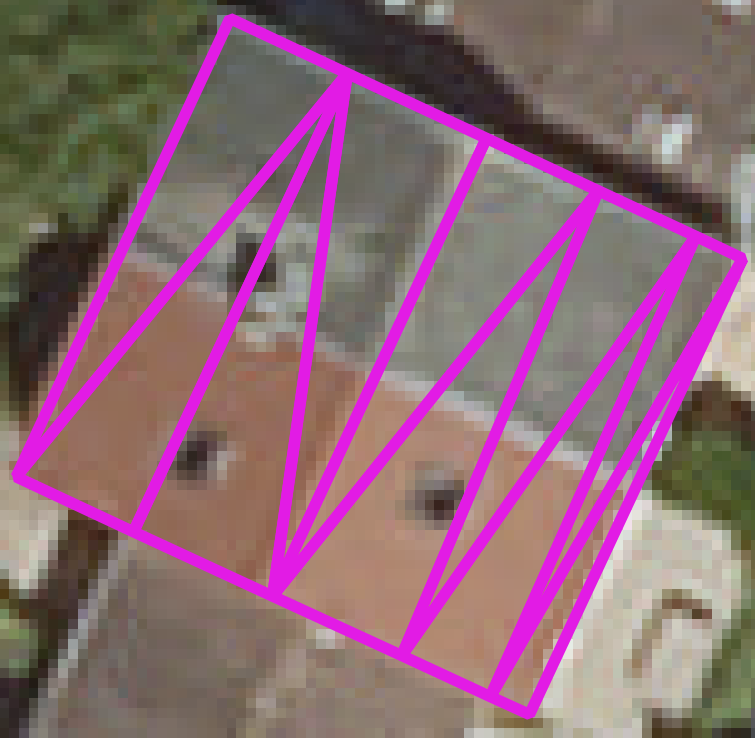
\includegraphics[height=.11\textheight]{images/Building_Errors/under_segmentation}}
                        \ffigbox[\FBwidth]{\caption{\textit{BOS}}\label{fig::over_bul}}{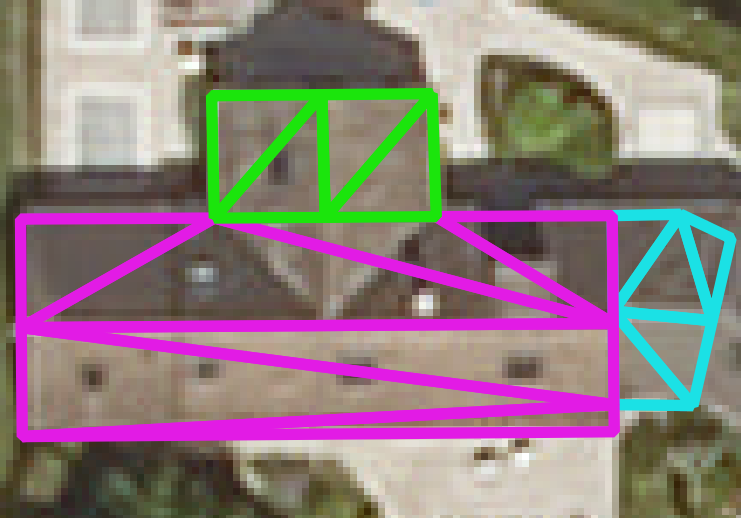
\includegraphics[height=.11\textheight]{images/Building_Errors/over_segmentation}}
                        \ffigbox[\FBwidth]{\caption{\textit{BInF}}\label{fig::footprint}}{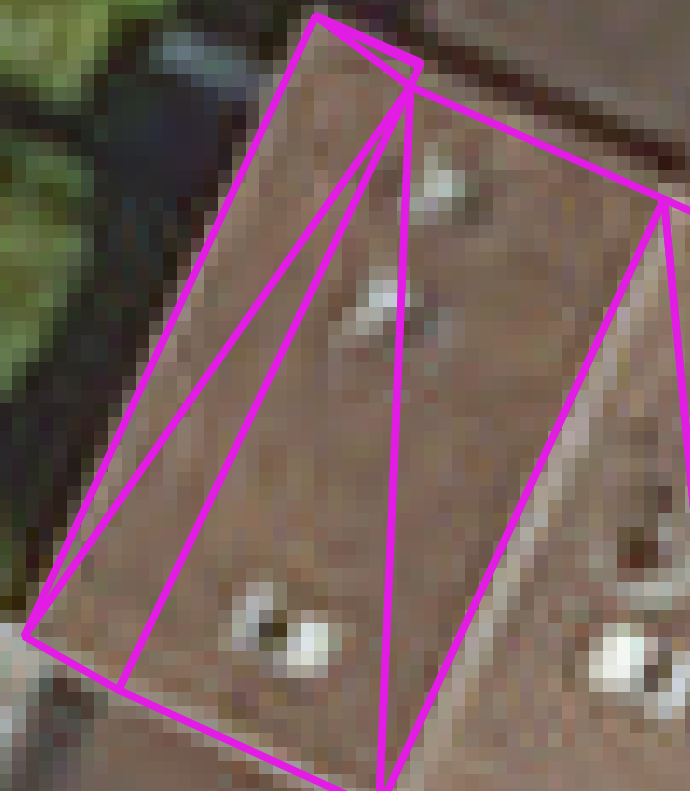
\includegraphics[height=.11\textheight]{images/Building_Errors/footprint}}
                        \ffigbox[\FBwidth]{\caption{\textit{BImH}}\label{fig::too_low}}{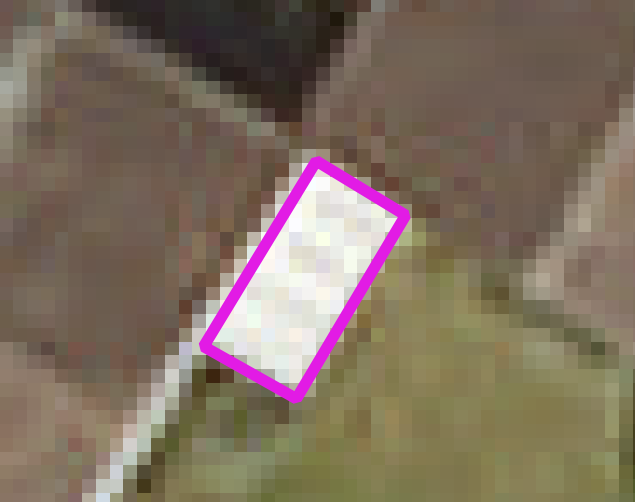
\includegraphics[height=.11\textheight]{images/Building_Errors/altimetric}}
                    \end{subfloatrow}
                }
                {
                    \captionsetup{labelfont={tiny, bf},textfont=scriptsize,justification=raggedright, labelsep=period}
                    \renewcommand{\thesubfigure}{\roman{SubFigCounter}}
                    \captionof{subfigure}{Building errors family samples.}\label{fig::bul_err}
                    \refstepcounter{SubFigCounter}
                    \addtocounter{figure}{-1}
                }
                \ffigbox[\FBwidth]
                {
                    \begin{subfloatrow}[4]
                        \ffigbox[\FBwidth]{\caption{\textit{FUS}}\label{fig::under_fac}}{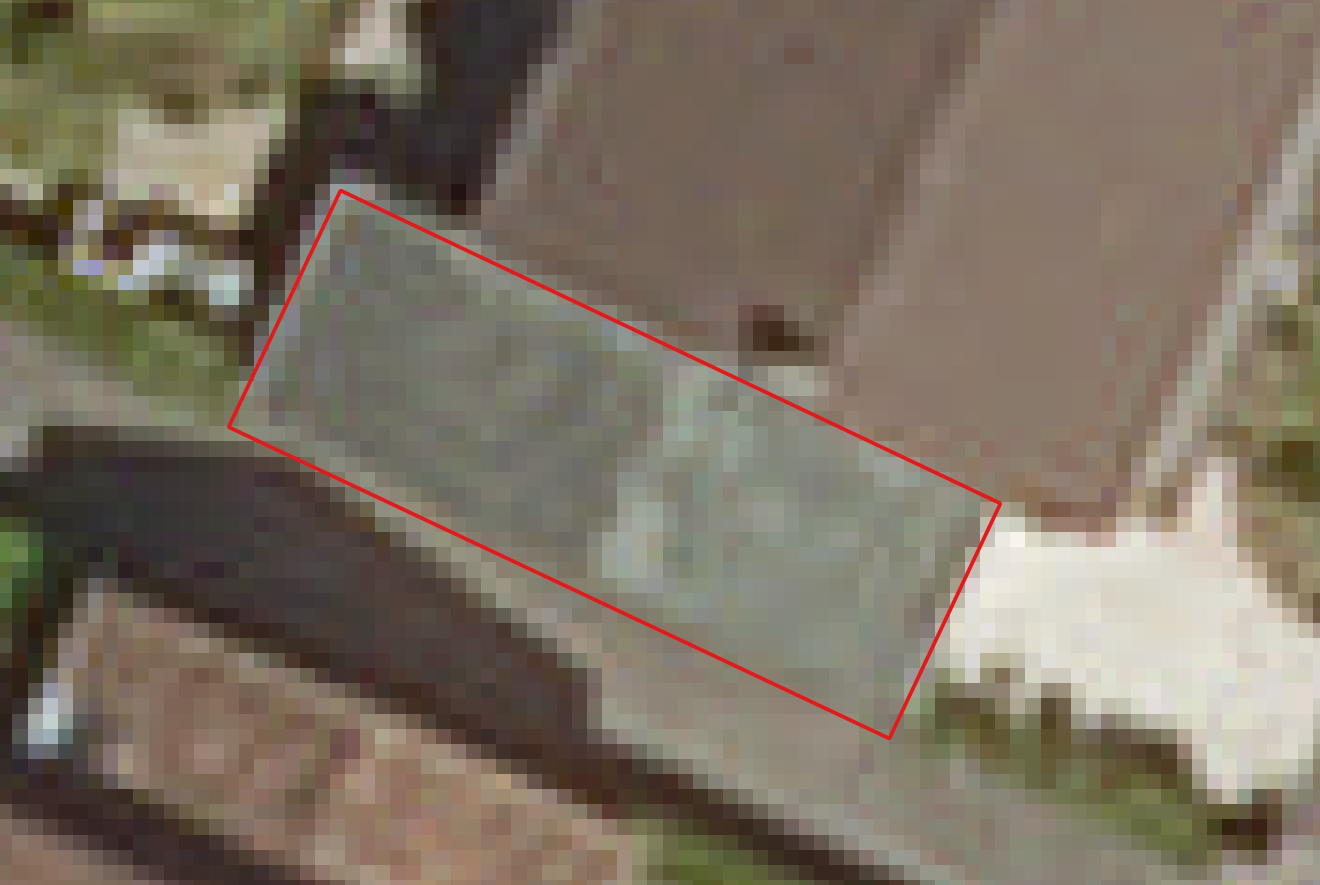
\includegraphics[height=.11\textheight]{images/Facet_Errors/under_segmentation}}
                        \ffigbox[\FBwidth]{\caption{\textit{FOS}}\label{fig::over_fac}}{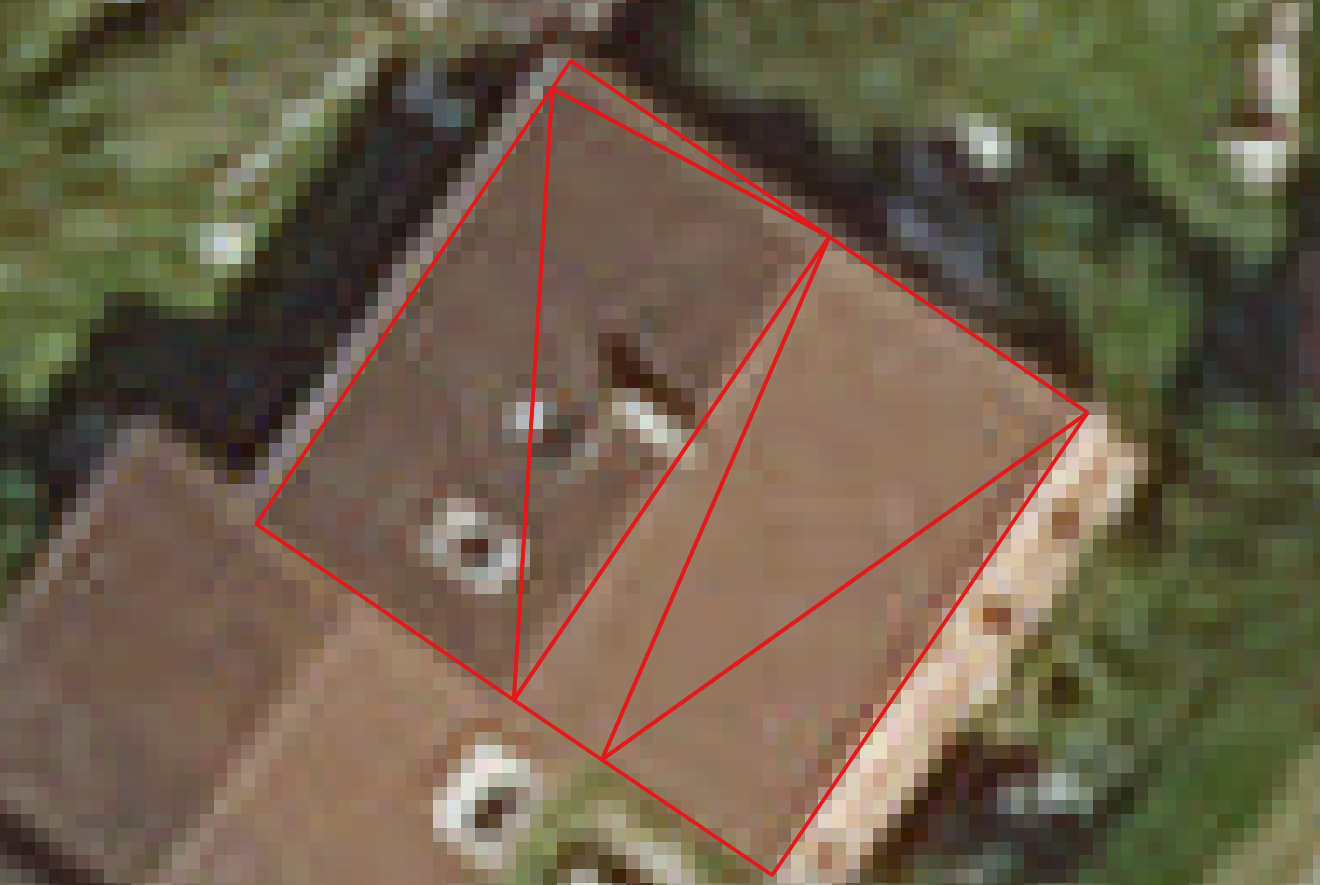
\includegraphics[height=.11\textheight]{images/Facet_Errors/over_segmentation}}
                        \ffigbox[\FBwidth]{\caption{\textit{FIS}}\label{fig::mis}}{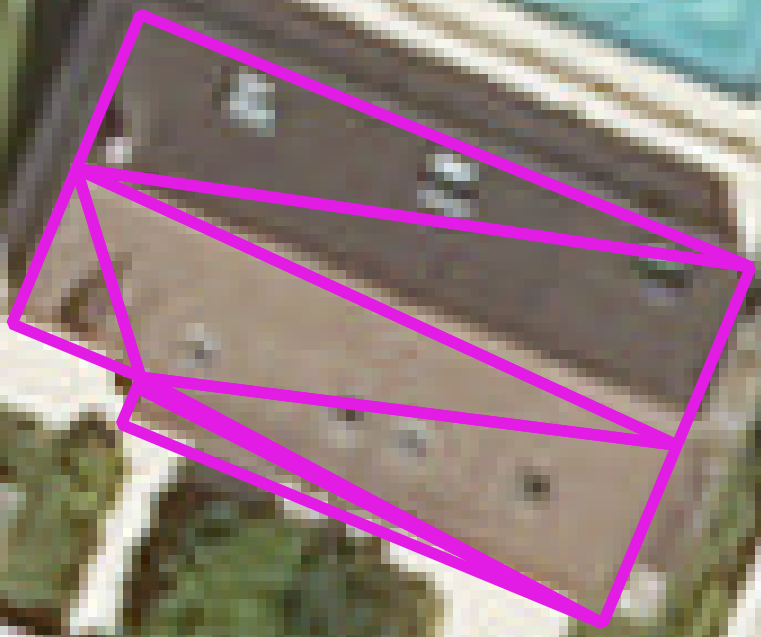
\includegraphics[height=.11\textheight]{images/Facet_Errors/mis_segmentation}}
                        \ffigbox[\FBwidth]{\caption{\textit{FImS}}\label{fig::slope}}{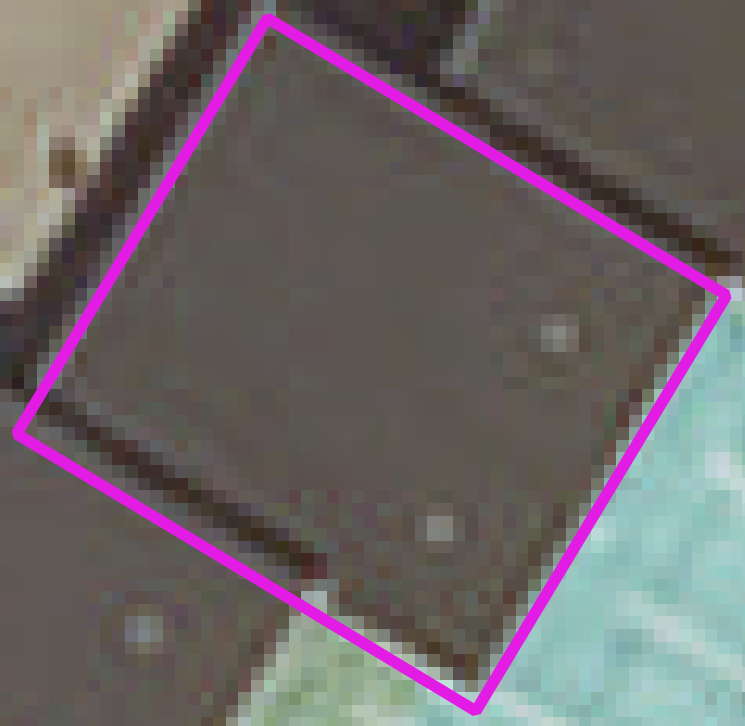
\includegraphics[height=.11\textheight]{images/Facet_Errors/slope}}
                    \end{subfloatrow}
                }
                {
                	\captionsetup{labelfont={bf},justification=raggedright, labelsep=period}
                    \renewcommand{\thesubfigure}{\roman{SubFigCounter}}
                    \captionof{subfigure}{Facet errors family samples.}\label{fig::fac_err}
                    \refstepcounter{SubFigCounter}
                    \addtocounter{figure}{-1}
                }
            }
            {
                \caption{\label{fig::samples}Illustration of various errors of our taxonomy. One can see that geometric, spectral and height information are required for an accurate detection of all kinds of errors.}
            }
        \end{center}
    \end{figure}

\subsection{Feature baseline}
In order to predict errors, models need to be described using relevant attributes. Since there is no comparable work that studies the previously defined errors, we propose a new baseline of features. They are kept simple so as to be used in most situations relying on generally available data. Indeed, they are based on depth map comparison, segment and image gradient pairing or the model intrinsic structural characteristics. We avoid computing and comparing $3D$ lines~\cite{Michelin2013}, correlation scores~\cite{boudet2006supervised} or, in general, any Structure-from-Motion (SfM) based metric~\cite{kowdle2011active}. In addition of being very costly, these features are methodologically endogamous to the $3D$ modeling techniques used to produce the assessed models. In other words, they are vulnerable to the same defects that may be overlooked during modeling in the first place.

The presented approach offers another flexibility lever related to the input data. The model itself can be directly used in order to discover flaws based on its geometrical structure compared to the dataset statistics. Dense depth information can be added, through for instance a \acrshort{acr::dsm}, in order to help detecting defects that can be hardly discriminated otherwise. Eventually, optical images can bring additional information critical for semantic heavy segmentation evaluation (high frequencies and texture). Each modality is described herein in detail.

\subsubsection{Geometric features.}
The model facet set is denoted by $\mathsf{F}$. $\forall (f, g) \in \mathsf{F} \times \mathsf{F} \quad f \sim g$ correspond to facets $f$ and $g$ being adjacent: \textit{i.e.}, they share a common edge. As the roof topology graph in~\cite{Verma2006}, the input building model can be seen as a facet (dual) graph:
\begin{equation}
	\label{eq::model_graph}
	\mathsf{M} \triangleq \Big(\mathsf{F}, \mathsf{E} \triangleq \big\{ (f, g) \in \mathsf{F} \times \mathsf{F} : f \sim g \big\} \Big).
\end{equation}
For each facet $f \in \mathsf{F}$, we compute its degree (\textit{i.e.}, number of vertices; $d(f) \triangleq \vert\{v : v\text{ is a vertex of }f\}\vert$), area $\mathscr{A}(f)$, circumference $\mathscr{C}(f)$, centroid $\mathscr{G}(f)$ and  normal $\vec{n}(f)$. Statistical characteristics are then computed over building model facets using specific functions $S$, like a histogram $S^p_{hist}: l \mapsto histogram(l, p)$, with $p$ standing for histogram parameters. Another simple option could be $S_{synth}: l \mapsto \begin{bmatrix}
\max(l)& \min(l) & \bar{l} & \text{median}(l) & \sigma(l)
\end{bmatrix}$ where $\bar{l}$ (\textit{resp.} $\sigma(l)$) represents the mean (\textit{resp.} the standard deviation) over a tuple $l$.

Each building $\mathsf{M}$ can consequently be characterized by a geometric feature vector that accounts for its geometric characteristics:

\begin{equation}
	\label{eq::geom_feat}
    v_{geometric}(\mathsf{M}) = \begin{bmatrix}
    	S \Big(\big(d(f)\big)_{f \in \mathsf{F}}\Big)\\
    	S \Big(\big(\mathscr{A}(f)\big)_{f \in \mathsf{F}}\Big)\\
    	S \Big(\big(\mathscr{C}(f)\big)_{f \in \mathsf{F}}\Big)\\
    	S \Big(\big( \vert\vert \mathscr{G}(f) - \mathscr{G}(g) \vert\vert \big)_{(f,g) \in \mathsf{E}}\Big)\\
    	S\Big(\big( \arccos(\vec{n}(f), \vec{n}(g)) \big)_{(f,g) \in \mathsf{E}}\Big)
    \end{bmatrix}.
\end{equation}
Additionally to individual facet statistics, regularity is taken into account by looking into adjacent graph nodes as in~\cite{Zhou2012}. Such features express only a small part of structural information. Taking this type of information into account would implicate graph comparisons which are not genuinely simple tasks to achieve. Since our objective is to build a baseline, this approach has not been considered for the moment.

\subsubsection{Height based features.}
For this modality, raw depth information is provided by a \acrlong{acr::dsm} as a $2D$ height grid $dsm$. It must have been produced around the same time of the $3D$ reconstruction so as to avoid probable temporal changes. It is compared to the model altimetry like in~\cite{Bredif2007},~\cite{zebedin2008fusion}. The latter is inferred from its facets plane equations. It is then rasterized into the image $alt$ at the spatial resolution of the $dsm$. Their difference reveals a discrepancy map that can be exploited for the prediction (cf. Figure~\ref{fig::pipeline}.c). A baseline approach is proposed relying on pixel values statistics computed using previously defined functions $S$.
\begin{equation}
	\label{eq::alti_feat}
    v_{height}(\mathsf{M}) = S\big( dsm - alt \big)
\end{equation}
Equation~\ref{eq::alti_feat} summarizes how building height based features are computed. Different from a root mean square metric~\cite{lafarge2012creating},~\cite{Poullis2013}, the histogram captures the the discrepancy distribution. However, as for the previous geometric attributes, structural information coming from the model is lost.

\subsubsection{Image features.} We can benefit from high frequencies existing in Very High Spatial Resolution optical images.
Building edges correspond to sharp discontinuities in images~\cite{ortner2007building}. The idea is to compare these edges to local gradients in order to look for inconsistencies. In an ideal setting, in an image $I$, gradients computed at pixels $g$ that intersect any segment $s$ from the building projection (\ref{fig::radio}) will almost be collinear with its normal. In consequence, we qualify, applying the same statistical functions $S$, the distribution of the normalized gradient scalar product with the normal all along a facet edge:
\begin{equation}
	\label{eq::corr_seg}
    \mathsf{D}_S(s, I) \triangleq S \bigg( \Big(\frac{\nabla I(g) \cdot \vec{n}(s)}{\Vert \nabla I(g)\Vert})_{g \in I \textrm{ and } g \cap s} \Big)\bigg).
\end{equation}

\begin{figure}
	\begin{center}
    	\floatbox{figure}{
            \begin{subfloatrow}[2]
                \ffigbox[\FBwidth]{\caption{\tiny A building model projection superimposed on the aerial image.}\label{fig::radio}}{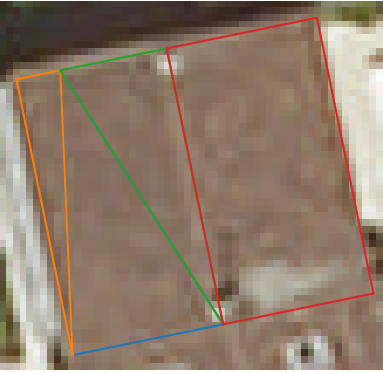
\includegraphics[width=.25\textwidth]{images/radio_vector}}
                \quad
                \ffigbox[\FBwidth]{\caption{\tiny The green squares represent intersecting pixels with the red segment. The gradient vector in purple is compared to the segment normal in black.}\label{fig::seg_inter}}{\includestandalone[mode=buildnew, width=.25\textwidth]{radiometric_features}}
            \end{subfloatrow}
        }{
        	\caption{Illustration of features that can be derived from optical images. For each model facet, the corresponding polygon projection edges are compared to local gradients as in (b).} \label{fig::image}
        }
	\end{center}
\end{figure}

Once the distribution is computed over a segment, it is compiled over all facet edges to define the distribution over projected facets. In the case of histograms $S_{hist}^p$ with the same parameters (and thus the same bins), it is equivalent to summing out the previous vectors $\mathsf{D}_{S_{hist}^p}(s, I)$ over segments $s$ forming the polygon projection $q(f)$ of the facet $f$ on as the image $I$. In order to take into account the variability of segment dimensions, this sum is weighted by segment lengths.
\begin{equation}
	\label{eq::corr_fac}
	D_{S_{hist}^p}(f, I) \triangleq \sum_{s \in q(f)} \Vert s \Vert \cdot \mathsf{D}_{S_{hist}^p}(s, I).
\end{equation}

The same can be done over all facets of a building $\mathsf{M}$, resulting in equation ~\ref{eq::corr_bul}. The weights are added in order to take into account the geometry heterogeneity. The gradient to normal comparison is similar to the $3D$ data fitting term formulation in~\cite{li2016boxfitting}. Once again, the model structure is partially lost when simply summing histograms over all segments.
\begin{equation}
	\label{eq::corr_bul}
	v_{image}(\mathsf{M}) = D_{S_{hist}^p}(\mathsf{M}, I) \triangleq \sum_{f \in \mathsf{F}} \mathscr{A}(q(f)) \cdot \mathsf{D}_{S_{hist}^p}(f, I).
\end{equation}

\subsection{Classification process}

When designing the classification process, two sources of flexibility are to be taken into account: the parametric nature of the taxonomy and the feature vector heterogeneity. The first means that labels to predict are not fixed but depend on the specified parameters. The second means that the classifier must adapt well to different input vectors types and sizes.

\noindent
\textbf{Classification problems.}
Both the classification problem nature and the set of labels to work with are determined by the three previously defined taxonomy parameters (cf. Table~\ref{tab::problems}). The first \textbf{target \textit{finesse}} $= 1$ level corresponds to a binary classification problem: ` `Valid'' or ``Erroneous''. At the next one $\textit{finesse}=2$, the other parameters intervene. The \textbf{\acrshort{acr::elod}} can take then two values in the aerial reconstruction case: \acrshort{acr::lod}-$1$ or \acrshort{acr::lod}-$2$. If fixed at \acrshort{acr::lod}-$1$, it is a binary classification problem: ``Valid'' or ``Building error''. For \acrshort{acr::lod}-$2$, if the \textbf{exclusivity} is on, it turns into a multi-class problem: ``Valid'', ``Building error'' or ``Facet errors'', while, if set off, it becomes a multi-label one: ``Valid'', ``Building error'' and ``Facet errors''. At the last $\textit{finesse}=3$ level, if the \textbf{exclusivity} is on, it is a $2$-stage classification problem. In the first stage, a multi-class, or simply binary in case $\acrshort{acr::elod} = \acrshort{acr::lod}1$, problem, like in the previous semantic degree, predicts the error family, after which a second multi-label problem decides between the predicted error family children. If the \textbf{exclusivity} is off, it changes into  $1$-stage multi-label problem that guesses the existence of each atomic error corresponding to the chosen \acrshort{acr::elod}.

\begin{table}
	\begin{center}
		\begin{tabular}{c c c x{8cm}}
			\toprule
            \textbf{\textit{finesse}} & \textbf{\acrshort{acr::elod}} & \textbf{exclusivity} & \textbf{Classification output}\\
            \midrule
            \scriptsize
            $1$ & -- & -- & Binary(Valid, Erroneous)\\
            $2$ & \acrshort{acr::lod}-$1$ & -- & Binary(Valid, Building error)\\
            $2$ & \acrshort{acr::lod}-$2$ & on & MultiClass(Valid, Building error, Facet error)\\
            $2$ & \acrshort{acr::lod}-$2$ & off & MultiLabel(Valid, Building error, Facet error)\\
            $3$ & \acrshort{acr::lod}-$1$ & on & MultiLabel(children(Binary(Valid, Building error)))\\
            $3$ & \acrshort{acr::lod}-$2$ & on & MultiLabel(children(MultiClass(Valid, Building error, Facet error)))\\
            $3$ & \acrshort{acr::lod}-$1$ & off & MultiLabel(children(Building error))\\
            $3$ & \acrshort{acr::lod}-$2$ & off & MultiLabel(children(Building error)$\cup$ children(Facet error))\\
            \bottomrule
		\end{tabular}
        \caption{\label{tab::problems} The summary of all possible classification problem types. children($error$) lists the children of $error$ from the taxonomy tree (Figure~\ref{fig::taxonomy}).}
	\end{center}
\end{table}

In a multi-class classification problem, each instance has only one label that takes only one value amongst multiple ones (two in the case of binary classification). The multi-label problem decides, for multiple labels, the most probable state: present ($+1$) or absent ($-1$). In the multi-stage setting, one decides, at each level, the most probable class or labels which impact the next stages of prediction. Errors are easily propagated in the last case. That is why, the rest of the study is not interested in this case. Since it focuses on semantic evaluation, the first \textit{finesse} degree is not experimented on. Furthermore, it can be inferred from higher levels of \textit{finesse}.

\noindent
\textbf{Classifier choice.} The highly modular nature of proposed features involving a great number of parameters restricts the choice of classifiers. Random forest classifiers~\cite{breiman2001random},~\cite{criminisi2013decision} were retained in this setting. In fact, they can manage a great number of features with different dynamics and coming from multiple modalities. Relying on their bagging property, a high number of trees ($1,000$ elements) is necessary to cover most of the feature space, while a limited tree depth ($4$) helps avoiding overfitting during training. It adapts also to any classification paradigm: multi-class or multi-label. In the latter case, a one-vs-all approach is adopted in addition so as to address each label separately.
\section{Experiments}
\label{sec:expe}
\subsection{Data}

We evaluate our approach using a 3D city model over the city of Elancourt (France). The studied scene spans an area of \SI{15}{\km\squared}. It exhibits a high diversity of building types and errors: residential districts with mostly bi-level buildings, industrial areas with flat roof buildings, a stadium, a petrol station and administrative edifices such as schools. These were modeled, using the algorithm described in~\cite{Durupt2006}, out of existing building footprints and an aerial multi-view \acrshort{acr::dsm} with a \SI{0.06}{\m} spatial resolution. The modeling algorithm simulates possible constrained roof structures. The best one is selected after scoring the extrapolated roofs. Finally, orthogonal building fa\c{c}ades connect the best roof to the ground. The produced $2.5D$ models have a \acrshort{acr::lod}-$2$ level. This method is adapted to roof types of low complexity and favors symmetrical models. Therefore, a high number of errors exist in our test case. $1,501$ buildings are considered in these experiments. They were annotated according to the atomic errors list provided by our taxonomy. Table~\ref{tab::statistics} reports statistics over the annotated dataset.

\begin{table}
    \scriptsize
    \begin{center}
        \begin{tabular}{|x{1.8cm} | x{1.8cm} | x{3cm} | x{2.8cm} | x{2.4cm}|}
            \hline
            \multicolumn{1}{|c|}{\textbf{Error Family}} & \textbf{Occurrence ratio} & \textbf{\emph{Atomic} error} & \textbf{Family conditional occurrence ratio} & \textbf{Absolute occurrence ratio} \\
            \hline
            Unqualifiable & $0.0180$ & --- & --- & --- \\
            \hline
            \hline
            \multirow{4}{*}{\shortstack{Building\\Errors}} & \multirow{4}{*}{$0.8235$} & Over segmentation & $0.8285$ & $0.6822$\\
            \cline{3-5}
                &                   & Under segmentation & $0.2824$ & $0.2325$ \\
            \cline{3-5}
                &                   & Imprecise footprint & $0.1521$ & $0.1252$ \\
            \cline{3-5}
                &                   & Imprecise height & $0.0057$ & $0.0047$ \\
            \hline
            \hline
            \multirow{4}{*}{Facet Errors} & \multirow{4}{*}{$0.7249$} & Over segmentation & $0.8971$ & $0.6502$ \\
            \cline{3-5}
                &                   & Under segmentation & $0.1314$ & $0.0953$ \\
            \cline{3-5}
                &                   & Imprecise segmentation & $0.1351$ & $0.9793$ \\
            \cline{3-5}
                &                   & Imprecise slope & $0.0193$ & $0.0140$ \\
            \hline
        \end{tabular}
        \caption{\label{tab::statistics} Ground truth statistics over the dataset containing $1501$ buildings. \textit{Atomic} errors are miscellaneously represented.}
    \end{center}
\end{table}

Both error families are highly present in the dataset. Only a small fraction ($27$ samples) of instances are unqualifiable, being occluded, completely or partially, by vegetation. At the atomic level, apart from building and facet over segmentation cases, most errors are under-represented with the extreme case of height imprecision error ($7$ samples). The unbalanced nature of our datasets obviously affects our results, as highlighted later in the next Section.
\subsection{Results}

\begin{table}
	\scriptsize
	\begin{center}
        \begin{tabular}{|x{1.4cm} | x{1.2cm} x{1.2cm} | x{1.2cm} x{1.2cm} | x{1.2cm} x{1.2cm} | x{1.2cm} x{1.2cm}|}
			\hline
            &\multicolumn{2}{x{2.4cm}|}{\textbf{Geometry}} & \multicolumn{2}{x{2.4cm}|}{\textbf{Geom. $\cup$ Height}} & \multicolumn{2}{x{2.4cm}|}{\textbf{Geom. $\cup$ Image}} & \multicolumn{2}{|x{2.4cm}|}{\textbf{All}}\\
            \cline{2-9}
            &\textbf{Recall} & \textbf{Prec.} & \textbf{Recall} & \textbf{Prec.} & \textbf{Recall} & \textbf{Prec.} & \textbf{Recall} & \textbf{Prec.}\\
            \hline
            Building errors & $99.76$ & \textbf{84.16} & $99.76$ & $84.11$& $99.92$ & $83.84$ & \textbf{100} & $83.85$ \\
            \hline
            Facet errors & $90.81$ & $98.02$ & \textbf{91.08} & \textbf{98.41} & $90.44$ & $97.62$ & $90.53$ & $97.82$ \\
            \hline
		\end{tabular}
	\end{center}
    \caption{\label{tab::f2_res}Test results expressed in percentage for the $\textit{finesse}=2$ case. All four configurations are compared across both family errors. \textbf{Geom.} stands for geometric}
\end{table}

Based on the devised pipeline, four feature configurations were tested: ``geometric features'' only, ``geometric and height features'', ``geometric and image features'' as well as ``geometric, height and image features''. Each feature modality produces a $20$ dimension vector. A \SI{0.06}{\m} spatial resolution \acrshort{acr::dsm} and a \SI{0.2}{\m} pixel size orthorectified image are used to derive height and image features. Labels are extracted from a non \textbf{exclusive} and \textbf{\acrshort{acr::elod}} $=$ \acrshort{acr::lod}-$2$ taxonomy. Both \textit{finesse} levels $2$ and $3$ are tested. We perform a $10$-fold cross validation. The overall accuracy is not interesting regarding the highly unbalanced nature of labels.
\begin{table}
	\scriptsize
	\begin{center}
        \begin{tabular}{|x{1.4cm} | x{1.2cm} x{1.2cm} | x{1.2cm} x{1.2cm} | x{1.2cm} x{1.2cm} | x{1.2cm} x{1.2cm}|}
			\hline
            &\multicolumn{2}{x{2.4cm}|}{\textbf{Geometry}} & \multicolumn{2}{x{2.4cm}|}{\textbf{Geom. $\cup$ Height}} & \multicolumn{2}{x{2.4cm}|}{\textbf{Geom. $\cup$ Image}} & \multicolumn{2}{|x{2.4cm}|}{\textbf{All}}\\
            \cline{2-9}
            &\textbf{Recall} & \textbf{Prec.} & \textbf{Recall} & \textbf{Prec.} & \textbf{Recall} & \textbf{Prec.} & \textbf{Recall} & \textbf{Prec.}\\
            \hline
            \textit{BOS} & \textbf{94.34} & $77.09$ &$93.36$ & \textbf{77.66} &$92.38$ & $77.04$ &$92.19$ & $76.69$ \\
            \hline
            \textit{BUS} & $34.38$ & $76.43$ &$31.52$ & \textbf{78.57} & \textbf{42.98} & $76.53$ &$41.55$ & $77.96$ \\
            \hline
            \textit{BInf} & \textbf{22.34} & \textbf{68.85} & $22.34$ & $67.74$ &$18.09$ & $64.15$ &$18.62$ & $64.81$ \\
            \hline
            \textit{BImH} & $0$ & --- & $0$ & --- & $0$ & --- &$0$ & $0$ \\
            \hline
            \hline
            \textit{FOS} & $98.77$ & \textbf{98.77} & \textbf{98.87} & $98.67$ &$98.67$ & $98.47$ &$98.67$ & $98.37$ \\
            \hline
            \textit{FUS} & \textbf{0.70} & \textbf{50.00} &$0.70$ & $33.34$ & \textbf{0.70} & \textbf{50.00} & \textbf{0.70} & \textbf{50.00} \\
            \hline
            \textit{FIS} & \textbf{1.36} & \textbf{66.67} &$1.36$ & $50.00$ &$1.36$ & $28.57$ &$1.36$ & $40.00$ \\
            \hline
            \textit{FImS} & $0$ & --- & $0$ & --- & $0$ & --- &$0$ & --- \\
            \hline
		\end{tabular}
	\end{center}
    \caption{\label{tab::f3_res}Test results reported in percentage for the \textit{finesse} level $3$. All \textit{atomic} errors are considered over all possible configurations. Ratios in bold represent the higher ones for each error.}
\end{table}
\subsection{Discussion}

Three criteria are considered when investigating qualitative results (Tables~\ref{tab::f2_res}-\ref{tab::f3_res}). The first analysis dimension involves \textit{finesse}. Scores are compared, between both \textit{finesse} levels, by averaging across all feature configurations. In terms of precision, at \textit{finesse} level $3$, compared to \textit{finesse} level $2$, ``Facet errors'' family looses $7.2\%$, while ``Building errors'' gains only $0.6\%$. The same \textit{finesse} level comparison reveals that recall is diminished by $2.0\%$ for ``Facet errors'' and $8.3\%$ for ``Building errors''. Thus, if limited to determining the error family, training the model at the \textit{finesse} level $2$ is the best alternative. Feature configurations are also studied in order to assess image and height attributes contributions. In general, results vary within a $2\%$ margin except in three cases. First, the precision instability for facet inexact and under segmentation can be spotted, as they are under detected: only one or two are rightfully identified as errors, while the number of valid instances, that are predicted as erroneous, vary between $1$ and $5$. Secondly, inexact footprint recall decreases by around $4\%$ in precision, when image features are added. This could result from the insufficient spatial resolution of optical images. However, in the last case, image features help ``Building under segmentation'' error gaining around $9\%$ in recall while loosing only $1.5\%$ in precision. This may be explained by the high radiometric heterogeneity of building roofs. Finally, scores are distinguished according to \textit{atomic} errors. As predicted, defects that are well represented in the dataset achieve high recall and precision values. The others, being present at rates lower than $23\%$, are not well predicted, especially in the case of very rare errors: height imprecision ($7$) or slope errors ($21$).

Qualitative assessment is also performed in order to illustrate some failure cases (Figure~\ref{fig::results}, from left to right). In the first image, the similarity of the building outline to over segmented buildings cases induces an overdetection. In the second example, the building is wrongfully detected as being under segmented due to the presence of a balcony and a smaller annex building. In the third building, while correctly predicting \textit{BOS}, our algorithm fails to detect the under segmented roof. Finally, in the last depiction, except the well caught footprint error, defects are overlooked as there are few comparable samples in the dataset. To alleviate these issues, more robust features could be introduced taking into account higher order information. Dataset enrichment could be another option which provides more instances of underrepresented errors. In the end, we can also add the human in the loop through manual interactive evaluation which can adapt well to user-specific needs.

\begin{figure}
	\begin{center}
    \tiny
		\begin{tabular}{| x{1.11cm} | x{.75cm} | x{.75cm} || x{1.11cm} | x{.75cm} | x{.75cm} || x{1.11cm} | x{.75cm} | x{.75cm} || x{1.11cm} | x{.75cm} | x{.75cm} |}
			\hline
			\multicolumn{3}{| c ||}{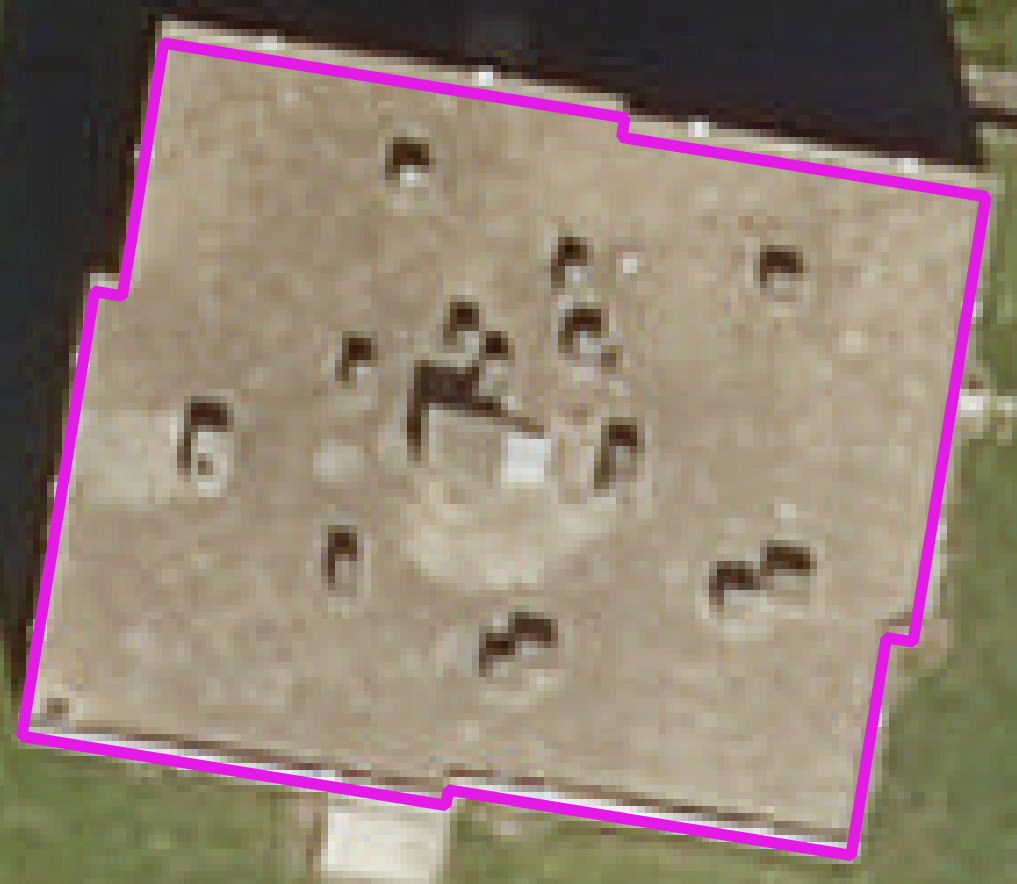
\includegraphics[height=.1\textheight,valign=m,margin=.1cm .1cm]{images/prediction_results/valid_as_bul_over}} & \multicolumn{3}{ c ||}{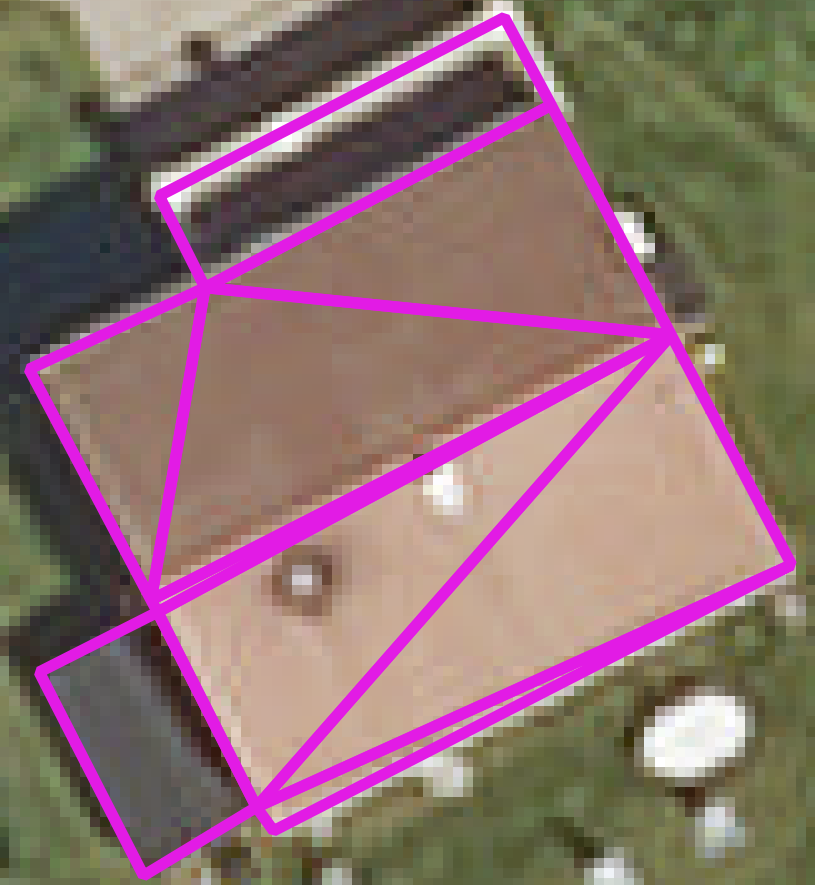
\includegraphics[height=.1\textheight,valign=m,margin=0cm .1cm]{images/prediction_results/no_imprec_no_fac_over}} & \multicolumn{3}{ c ||}{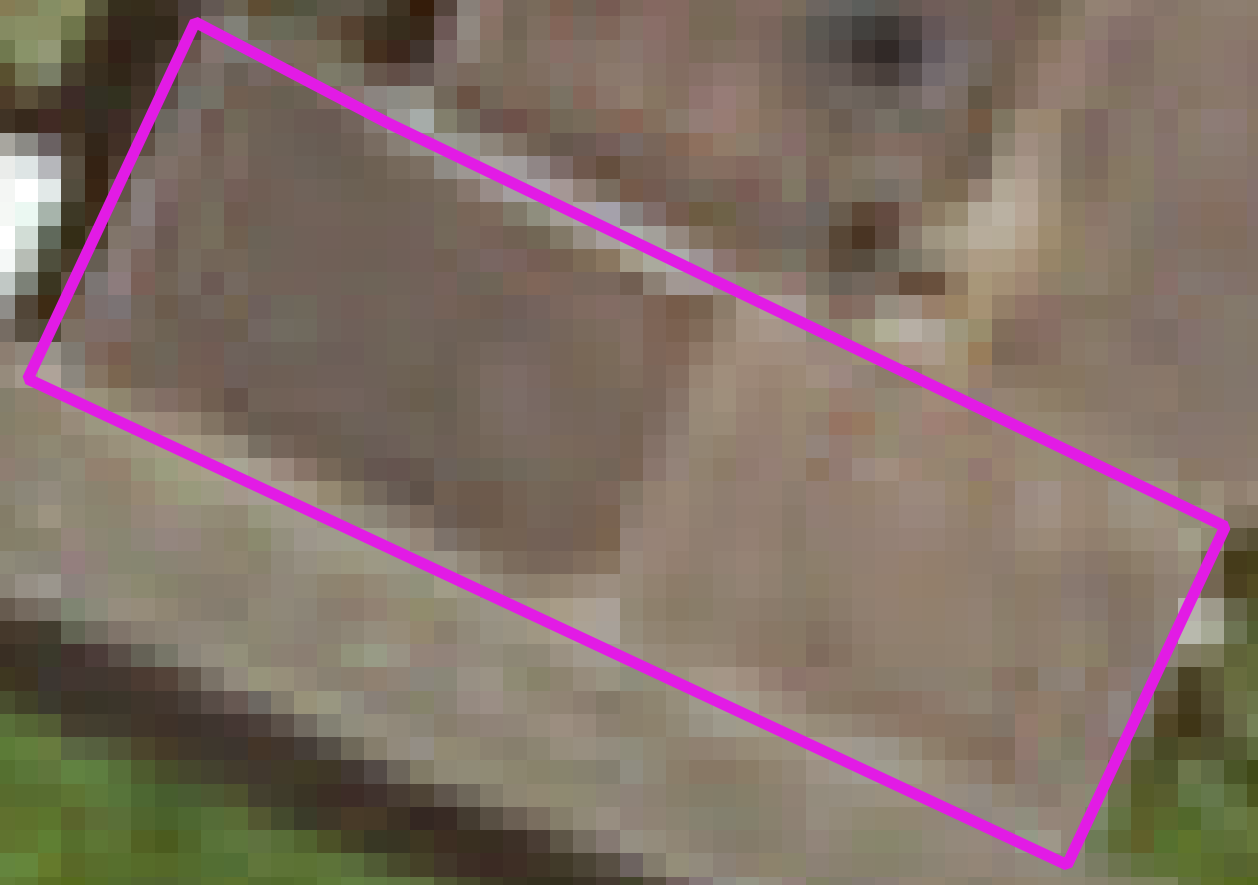
\includegraphics[height=.1\textheight,valign=m,margin=0cm .1cm]{images/prediction_results/no_under_seg}} & \multicolumn{3}{ c |}{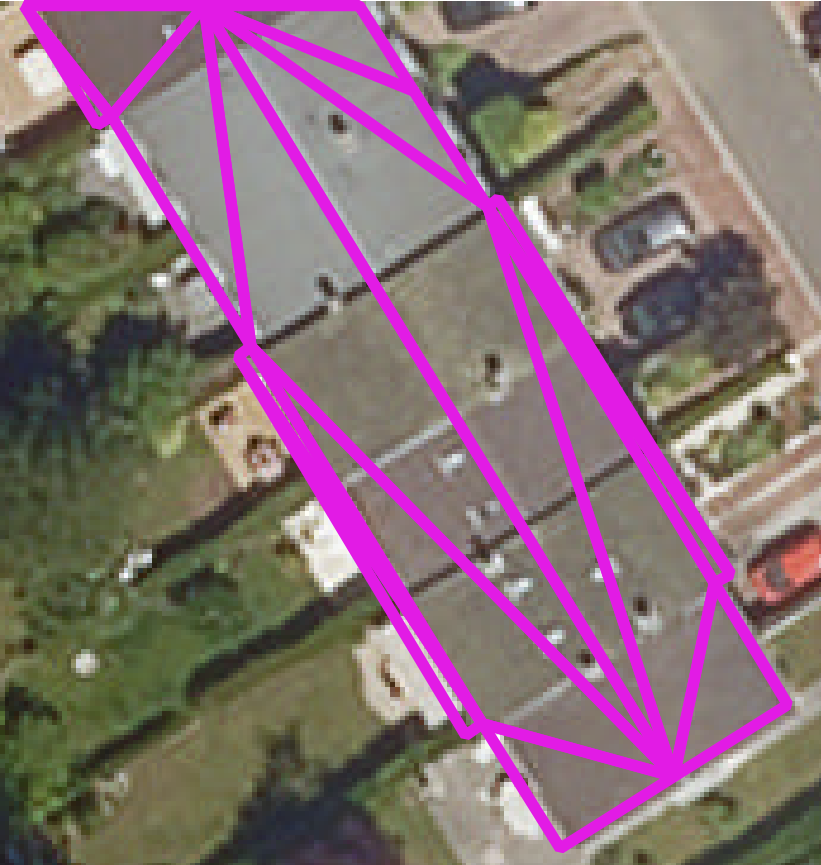
\includegraphics[height=.1\textheight,valign=m,margin=0cm .1cm]{images/prediction_results/no_bul_under_seg}} \\
			\hline
			\textbf{Errors} & \textbf{G.T.} & \textbf{Pred.} & \textbf{Errors} & \textbf{G.T.} & \textbf{Pred.} & \textbf{Errors} & \textbf{G.T.} & \textbf{Pred.} & \textbf{Errors} & \textbf{G.T.} & \textbf{Pred.}\\
            \hline
            \textit{BOS} & \xmark & \cmark & \textit{BUS} & \xmark & \cmark & \textit{BOS} & \cmark & \cmark & \textit{BOS} & \cmark & \xmark \\
            Valid & \cmark & \xmark & \textit{FImS} & \cmark & \xmark & \textit{FUS} & \cmark & \xmark &  \textit{FOS} & \cmark & \xmark \\
             &  &  & \textit{FOS} & \cmark & \xmark &  &  &  & \textit{BUS} & \cmark & \xmark \\
             &  &  &  &  &  &  &  &  &  \textit{BInF} & \cmark & \cmark \\
            \hline
		\end{tabular}
        \caption{\label{fig::results} Predicted (Pred.) errors compared to ground truth (G.T.) labels are illustrated for some pathological cases. Knowing how each error is represented in the dataset helps interpreting mispredictions.}
	\end{center}
\end{figure}

\section{Conclusion}
\label{sec::conclusion}

We proposed a framework to semantically evaluate automatically modeled buildings. For that purpose, errors are hierarchically organized into a flexible and parametrized taxonomy. It aims to handle the large diversity of urban enviroments and varying requirements stemming from end-users (geometric accuracy and level of details). Based on the desired \acrshort{acr::lod}, exclusivity and semantic level, an error collection is considered. Model quality is then predicted using a supervised classifier. Each model provides intrinsic geometrical characteristics that are compiled in a feature vector. Other modalities can help describing building models, as attributes can also be extracted from model comparison to images or depth data. It helps detecting hard cases.

This new framework was applied to the case of aerial urban reconstruction, where features are extracted from geospatial images and a \acrshort{acr::dsm}. A dataset containing $1,501$ aerial reconstructed building models with high diversity was used to test the devised evaluation method associated to multimodal baseline features. Although being mitigated over under-represented errors, results are satisfactory in the well balanced cases. As a next step, more structurally aware features (based on graph comparison, for instance) could be proposed so as to be applied on a richer and more diverse dataset (potentially involving data augmentation) under a deep-based framework.
\bibliographystyle{splncs}
\bibliography{references}
\end{document}
